\documentclass[11pt,oneside]{article}
\input{coursHeadings}
\usepackage[raccourcis]{FAST}
\usepackage[%
    pdftitle={Produits Procédés Matériaux -- },
    pdfauthor={Xavier Pessoles},
    colorlinks=true,
    linkcolor=blue,
    citecolor=magenta]{hyperref}

\usepackage{pifont}


% \makeatletter \let\ps@plain\ps@empty \makeatother
%% DEBUT DU DOCUMENT
%% =================
\sloppy
\hyphenpenalty 10000

\newcommand{\Pointilles}[1][3]{%
\multido{}{#1}{\makebox[\linewidth]{\dotfill}\\[\parskip]
}}


\colorlet{shadecolor}{orange!15}

\newtheorem{theorem}{Theorem}


\begin{document}


\newboolean{prof}
\setboolean{prof}{true}
%------------- En tetes et Pieds de Pages ------------
\pagestyle{fancy}
\renewcommand{\headrulewidth}{0pt}

\fancyhead{}
\fancyhead[L]{%
\noindent\noindent\begin{minipage}[c]{2.6cm}
%Lycée Rouvière PTSI
\includegraphics[width=2cm]{png/logo_ptsi.png}%
\end{minipage}
}


\fancyhead[C]{\rule{12cm}{.5pt}}

\fancyhead[R]{%
\noindent\begin{minipage}[c]{3cm}
\begin{flushright}
\footnotesize{\textit{\textsf{Sciences Industrielles\\ de l'Ingénieur}}}%
\end{flushright}
\end{minipage}
}

\renewcommand{\footrulewidth}{0.2pt}

\fancyfoot[C]{\footnotesize{\bfseries \thepage}}
\fancyfoot[L]{\footnotesize{2012 -- 2013} \\ X. \textsc{Pessoles}}
\ifthenelse{\boolean{prof}}{%
\fancyfoot[R]{\footnotesize{Cours -- CI 6 : PPM -- P}}
}{%
\fancyfoot[R]{\footnotesize{Cours -- CI 6 : PPM}}
}



\begin{center}
 \huge\textsc{CI 6 -- PPM -- Produits Procédés Matériaux}

 \large\textsc{Élaboration des pièces mécaniques. Introduction de la chaîne numérique.}
\end{center}

\begin{center}
 \LARGE\textsc{Chapitre 11 -- Usinage -- Étude de la coupe}
\end{center}

\begin{flushright}
\textit{D'après documents de Jean-Pierre Pupier}
\end{flushright}

\vspace{.5cm}


\begin{minipage}[c]{.45\linewidth}
\begin{center}
\includegraphics[height=3cm]{png/copeau}

\textit{Modélisation de la formation du copeau\footnote{\url{http://www.geniemeca.fpms.ac.be}}}
\end{center}
\end{minipage} \hfill
\begin{minipage}[c]{.45\linewidth}
\begin{center}
\includegraphics[height=4cm]{png/copeau2}

\end{center}
\end{minipage} 
\vspace{.25cm}

A l'interface entre la pièce et l'outil, se produisent des phénomènes complexes dont l'outil est le principal acteur. Ce sont les phénomènes de coupe. Il importe donc de connaître :
\begin{itemize}
\item les principaux matériaux constitutifs des outils;
\item les phénomènes d'usure;
\item la géométrie des outils;
\item les efforts s'exerçant sur ces derniers.
\end{itemize}

%\begin{center}
%\includegraphics[width=.9\textwidth]{png/cyclev.png}

%\textit{Cycle de conception d'un produit}
%\end{center}

%\begin{prob}
%\textsc{Problématique :}
%\begin{itemize}
%\item %Quelles sont les conditions fonctionnelles permettant le fonctionnement du système ?
%\item %Quelle est la chaîne de côte unidirectionnelle correspondant à une condition donnée ?
%\end{itemize}
%\end{prob}



\begin{savoir}
\textsc{Savoirs :}
\begin{itemize}
\item Connaître la technologie élémentaire des éléments coupants (géométrie, matériaux)
\item Définir une puissance de coupe
\end{itemize}
\end{savoir}
 

\setlength{\parskip}{0ex plus 0.2ex minus 0ex}
 \renewcommand{\contentsname}{}
 \renewcommand{\baselinestretch}{1}

\tableofcontents

 \renewcommand{\baselinestretch}{1.2}
\setlength{\parskip}{2ex plus 0.5ex minus 0.2ex}

% \vspace{1cm}
\textit{Ce document évolue. Merci de signaler toutes erreurs ou coquilles.}

\section{Les matériaux à outils}





\subsection{Analyse du besoin d'un outil}
Pour avoir une bonne tenue à la coupe on demande principalement à un outil : 
\begin{itemize}
\item la dureté à froid et surtout la dureté à chaud;
\item la résistance à l'usure;
\item la ténacité (possibilité de se déformer avant rupture et résistance à la déformation plastique).
\end{itemize}

Il peut être également tenu compte de :
\begin{itemize}
\item l'usinabilité (problème d'affûtage);
\item la conduction thermique;
\item la résistance à l'oxydation et à la décarburation;
\item l'indéformabilité.
\end{itemize}

\subsection{Matériaux des outils}

\subsubsection{Les aciers rapides}
Ce sont des aciers fortement alliés dont la teneur en carbone dépasse 0,7\%. Ces aciers sont trempés. 

Leur domaine d'emploi va du travail d'ébauche à la finition quel que soit le type de machines. Actuellement ils sont la plupart du temps remplacés par les outils en carbure sauf dans le cas des outils de forme à profil complexe. Il est en effet possible de les affûter grâce à une meule. Leur vitesse « standard éducation nationale » de coupe est de 25 m/min pour l'usinage des aciers courants.

\paragraph*{Les différents éléments d'addition des aciers rapides}

\begin{center}
\begin{tabular}{|c|c|c|p{.6\textwidth}|}
\hline
Élément & Symbole & Pourcentage & Influence \\ \hline
Carbone & $C$& 1,75\% maxi & Influe sur la dureté au détriment de la ductilité.\\ \hline
Tungstène & $W$ & 6 à 18\% & Donne une bonne résistance à l'usure, affine le grain et maintient la dureté à chaud.\\ \hline
Molybdène & $Mo$ & 0,5\% à 9\% & Remplace le tungstène. Il permet d'obtenir une meilleure ductilité mais l'acier devient sensible à la décarburation et la fourchette de trempe sera plus étroite. \\ \hline
Vanadium & $V$ & 1 à 5\% & Élément d'alliage le plus important car il forme avec le carbone un carbure plus dur que les autres ce qui permet d'avoir une grande résistance à l'usure. \\ \hline
Chrome & $Cr$ & 4\%  & Influe la capacité de trempe de l'acier et sa résistance au revenu.\\ \hline
Cobalt  & $Co$ & 5 à 10\% & Permet d'augmenter la dureté à chaud.\\ \hline
Manganèse & $Mn$& & Évite les déformations des aciers.\\ \hline
\end{tabular}
\end{center}


\subsubsection{Les carbures}
Ce sont des carbures métalliques frittés pour la plupart. La dureté est proche de celle du diamant. Ce sont les outils d'aujourd'hui. De plus le système de plaquettes jetables permet des gains de productivité appréciables : plus d'affûtage, outil pouvant se passer d'être réglé après un changement d'arête de coupe, paramètres de coupe constants sur toute une série de pièces. Leur vitesse de coupe « moyenne et usuelle » est de $100\; m/min$ pour les aciers courants. Il y a toujours intérêt à compulser les documents des fabricants de carbure pour avoir des « valeurs industrielles » ($Vc$ pour une durée de vie de 15 minutes dans de l'acier $XC48$ peut en finition atteindre $300\; m/min$).

\paragraph{Les composants}
Le carbure a une dureté presque équivalente à celle du diamant et conserve ses caractéristiques à une température voisine de 1000\degre C.
	
Le carbure métallique est un produit fabriqué selon les techniques de la métallurgie des poudres. Deux constituants principaux entrent dans la composition des carbures métalliques, les substances et les liants métalliques.

Ces deux composants sont broyés en une proportion déterminée dans des broyeurs à boulets. Après addition de lubrifiant la poudre soigneusement broyée est pressée et subit l'opération de pré-frittage. Les pièces ont alors une consistance crayeuse donc fragile, mais permettant à ce stade de la fabrication de les façonner sans difficulté. 

Le produit pré-fritté subit alors une cuisson durant laquelle les carbures vont se lier de façon fine grâce au liant métallique. En effet seul ce dernier fond. On obtient alors le carbure final.

\paragraph{Les substances dures (phase $\alpha$ et phase $\gamma$)}
Elles composent 70 à 90\% du carbure, elles donnent la dureté et par suite la résistance à l'usure.

Elles se divisent en deux groupes appelés phases :
\begin{itemize}
\item phase $\alpha$ :
\begin{itemize}
\item WC : carbure de tungstène majoritairement (Température de fusion : 2600 \degre C)
\end{itemize}
\item phase $\gamma$ :
\begin{itemize}
\item $TiC$ : carbure de titane (Température de fusion : 3169 \degre C)
\item $TaC$ : carbure de tantale (Température de fusion : 3760 \degre C)
\item $NbC$ : carbure de niobium (Température de fusion : 3500 \degre C)
\end{itemize}
\end{itemize}


\paragraph{Les substances liantes (phase $\beta$)}

Elles représentent 10 à 30\% de la composition du carbure. Elles donnent la ténacité du carbure.
	
La plus employée est le cobalt car il dissout facilement les différents carbures. Il existe également le nickel et le fer.



\paragraph{Détermination des nuances}
La norme I.S.O. prévoit de classer les carbures en fonction du rapport substances liantes, substances dures. On obtient ainsi une classification en 3 lettres P, K, M, tenant compte de la dureté ou de la ténacité croissante.

Elle prévoit aussi une classification numérale pour compléter la classification littérale du type 01, 10,20, ..., 50, en fonction du domaine d'application.
 
\begin{center}
\includegraphics[width=.8\textwidth]{png/fig_01}
\end{center}

\subsubsection{Les céramiques}
Elles sont constituées de 90\% d'$Al_2O_3$ (alumine) et de 10\% d'oxyde métallique. Elles se révèlent surtout utiles pour des enlèvements importants de matière. Mais l'outil céramique supporte mal les variations importantes de copeau ce qui limite son utilisation pour des opérations de demi-finition où son action aura été préparée par un chanfrein d'entrée et un dégagement en fin d'usinage. La vitesse de coupe « standard » est de $500\; m/min$ pour un acier courant.

\subsubsection{Les outils revêtus}
Pour bénéficier à la fois des qualités équivalentes à celles des céramiques sans en avoir les inconvénients, on fabrique des plaquettes en carbure métallique pouvant être, entre autres, revêtues de céramique, de nitrure de titane, etc.

\subsubsection{Les diamants}
Réservés à la super finition, ils utilisent la grande dureté du carbone pur.


\subsection{Désignation des plaquettes et des portes plaquettes}
La désignation des portes plaquettes et des plaquettes fait l'objet d'une norme I.S.O. dont des éléments sont donnés ci-après.
\subsubsection{Portes plaquettes}
 
\begin{center}
\includegraphics[width=.8\textwidth]{png/fig_02}
\end{center}
\subsubsection{Plaquettes}

\noindent \begin{minipage}[c]{.45\linewidth}
\begin{center}
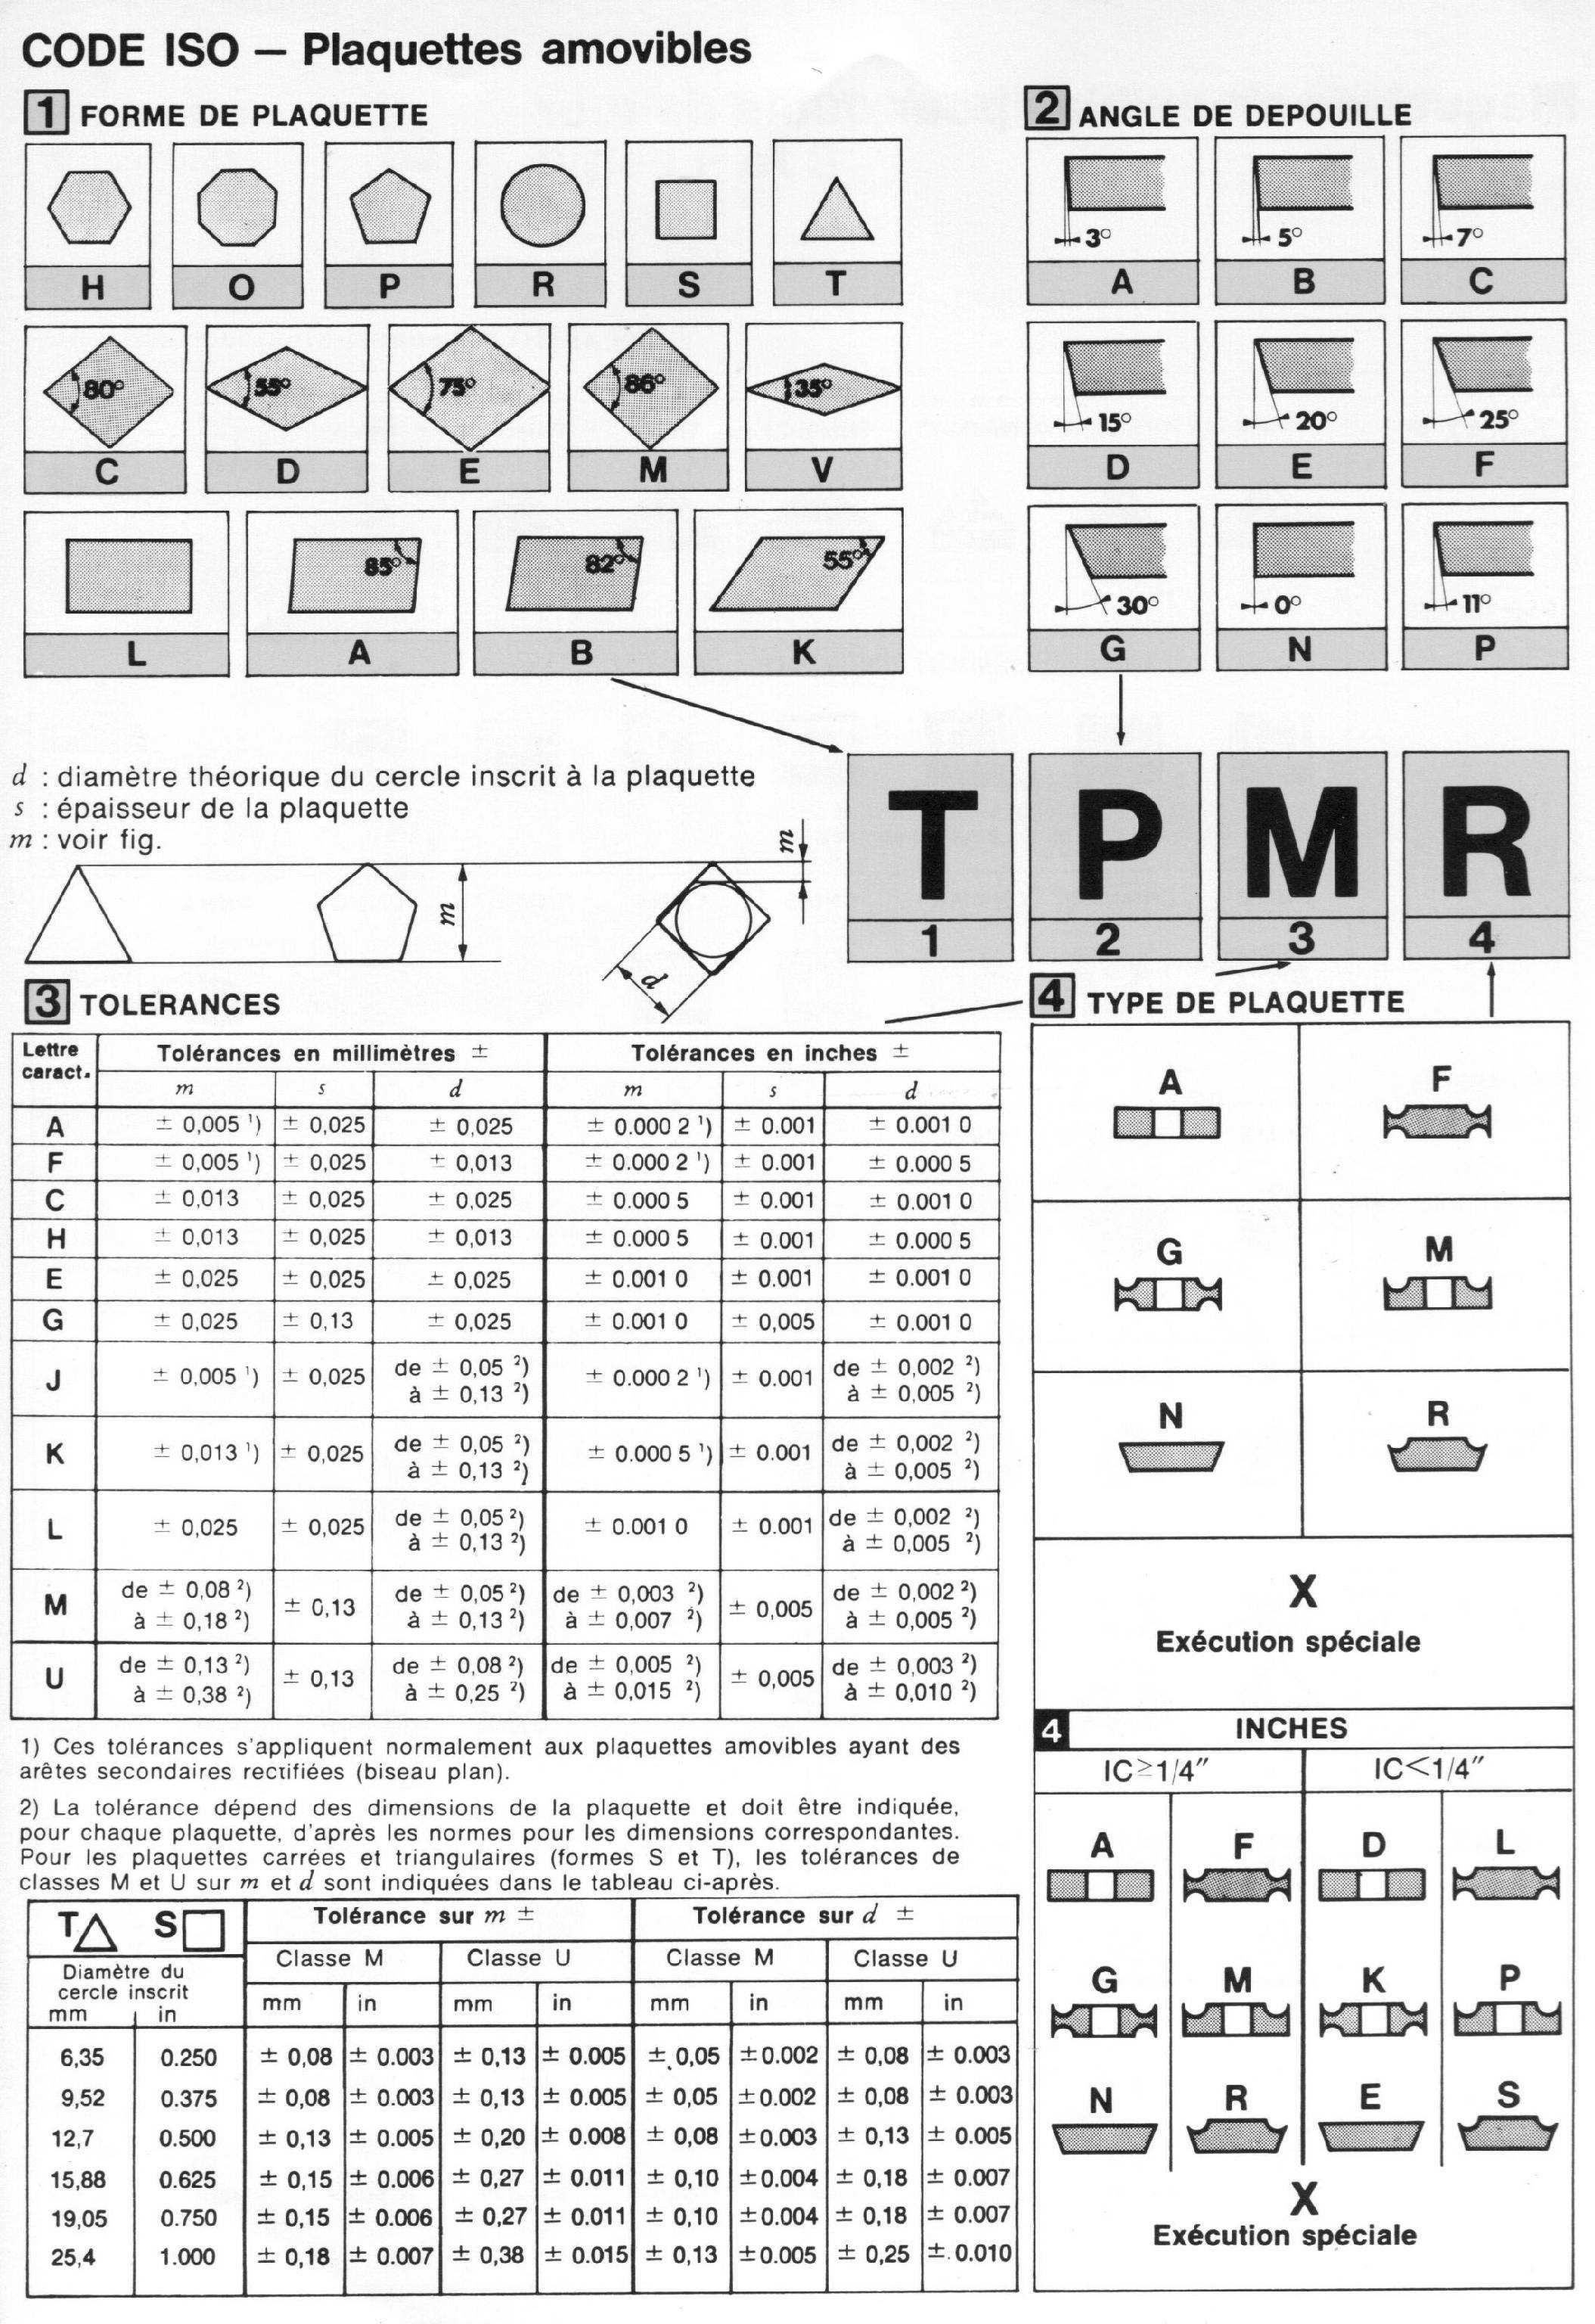
\includegraphics[width=\textwidth]{png/fig_03_1}
\end{center}
\end{minipage}\hfill
\begin{minipage}[c]{.45\linewidth}
\begin{center}
\includegraphics[width=\textwidth]{png/fig_03_2}
\end{center}
\end{minipage}

\section{L'usure des outils}

\subsection{Pourquoi l'étude de cette usure est-elle importante ?}

La coupe est l'interaction de deux matériaux, celui de l'outil et celui de la pièce, dont chacun a des caractéristiques géométriques propres au moment de la formation du copeau.
	
Il est évident que seule l'arête de l'outil est en contact permanent avec la pièce et c'est donc elle qui définit en priorité la géométrie de la pièce que l'on est en train d'usiner.
	
Il faut donc que cette arête garde un dimensionnement constant sinon la surface fabriquée sera hors tolérance : de plus il faut que son aptitude à la coupe soit maintenue sinon l'état de surface obtenu sera incorrect.

En limitant  la vitesse de coupe il est sûr que l'on pourra limiter l'usure de l'outil mais il est impératif pour le fabriquant de produire un maximum le plus rapidement possible pour des raisons impérieuses de rentabilité (produire le plus de pièces possible au meilleur coût dans les délais prévus).
	
L'étude de la coupe est donc fondamentale et une modélisation mathématique permet de quantifier les usures d'outils. 

\subsection{Les mécanismes de l'usure}
\subsubsection{La formation du copeau (étude simplifiée)}

\begin{center}
\includegraphics[width=.75\textwidth]{png/fig_04}
\end{center}

\subsubsection{Notion de brise-copeau}


\noindent \begin{minipage}[c]{.45\linewidth}
\begin{center}
\includegraphics[width=\textwidth]{png/fig_05}
\end{center}
\end{minipage}\hfill
\begin{minipage}[c]{.45\linewidth}
Le déroulement continu du copeau est gênant : il faut le fractionner. C'est le rôle du brise-copeau qui est réalisé par aménagement des formes de la face de coupe.
\end{minipage}




\subsection{Les manifestations de l'usure}

\noindent \begin{minipage}[c]{.45\linewidth}
\begin{center}
\includegraphics[width=.75\textwidth]{png/fig_06}
\end{center}
\end{minipage}
\begin{minipage}[c]{.45\linewidth}
Suivant les conditions de coupe (vitesse de coupe, couple matériau -- outil, couple matériau -- pièce, vitesse d'avance, profondeur de passe, etc.), les manifestations de l'usure sont différentes et ont donc été répertoriées (et normalisées pour certaines) pour pouvoir procéder à des comparaisons.
\end{minipage}

%
%\subsubsection{L'usure mécanique}
%
%Durant la coupe la surface de l'outil et la surface de la matière ne sont pas parfaitement en contact : seuls quelques points encaissent tous les efforts et la pression est telle qu'il y a création d'une soudure en phase solide. Le rapport entre surface réelle de contact et surface apparente de contact peut atteindre $10^{-5}$.
%

%					
%Le matériau de la pièce n'est pas forcément homogène et présente des particules dures. Ces dernières lors de l'usinage sont mises à nu et de ce fait jouent le rôle d'abrasif pour l'outil. Ces particules dures finissent par se détacher et véhiculées par le lubrifiant de coupe vont continuer à agir à l'interface outil pièce.
%
%
%........................
%
%
%
%L'outil est un conglomérat de particules dures. La liaison entre les grains de l'outil est sollicitée de façon cyclique et donc soumise à des contraintes de fatigue ce qui entraîne à la longue le détachement de ces particules.
%
%..............................
%
%\subsubsection{Usure par effets physico-chimiques}
%
%A partir d'une certaine température il y a migration de certains composants de l'outil, vers la pièce ce qui entraîne un changement des caractéristiques de ce dernier. Le phénomène est d'autant plus criant que la température de coupe augmente.
%
%...............................
%
%Dès qu'un matériau est en présence de certains corps ou gaz il y a possibilité de réactions chimiques dont la plus caractéristique sera l'oxydation de l'outil au contact de l'air et/ou au contact des fluides de coupe.
%
%................................
%
%\subsubsection{Conclusion : diagramme de Optis, Koening et Vieregge}
%
%Sur ce diagramme sont portées les différentes usures et les températures auxquelles elles se produisent. Quand on examine ce graphique il apparaît qu'aux faibles vitesses de coupe c'est l'usure adhésive qui prédomine. Avec l'augmentation de la vitesse de coupe donc de la température à l'interface outil/pièce, le matériau change de comportement et ce type d'usure diminue. Par contre l'usure par diffusion qui apparaît alors augmente dans de fortes proportions et devient le phénomène prépondérant.
%
%
%
%
%\subsection{Les manifestations de l'usure}
%
%Suivant les conditions de coupe - vitesse de coupe, couple matériau outil matériau pièce, vitesse d'avance, profondeur de passe, etc., les manifestations de l'usure sont différentes et ont donc été répertoriées, normalisées pour certaines pour pouvoir procéder à des comparaisons.
%


\subsubsection{L'usure en cratère $Kt$}

Elle apparaît pour les outils en carbure ou en céramique lors des travaux d'ébauche pour lesquels la pression de coupe est importante et la vitesse de coupe peu élevée, souvent pour des questions de puissance machine. Le copeau "appuie" sur la face de coupe en ménageant l'arête de coupe mais en « creusant » au-delà. Cela finit par entraîner «l’affaiblissement » de l'outil et sa destruction. 


\noindent \begin{minipage}[c]{.45\linewidth}
\begin{center}
\includegraphics[width=\textwidth]{png/fig_07}
\end{center}
\end{minipage}\hfill
\begin{minipage}[c]{.45\linewidth}
\begin{itemize}
\item $Kb$ : largeur du cratère;
\item $Km$ : distance du centre du cratère;
\item $Kt$ : profondeur du cratère;
\item $\gamma_c$ : angle de cratérisation.
\end{itemize}
\end{minipage}



			
\subsubsection{L'usure en dépouille $Vb$}

Elle apparaît pour des vitesses de coupe importantes dans le cadre de travaux de finition. Elle est due au frottement pièce outil et, provoquant le recul du point ou de l'arête générant la surface, change le dimensionnement de la pièce ainsi réalisée. D'autre part les angles de coupe n'étant plus respectés il y a détérioration de l'état de surface.

\noindent \begin{minipage}[c]{.45\linewidth}
\begin{center}
\includegraphics[width=.8\textwidth]{png/fig_08}
\end{center}
\end{minipage}\hfill
\begin{minipage}[c]{.45\linewidth}
\begin{itemize}
\item Zone C : partie pointe de l'outil partie courbe de l'arête
\item Zone N : 1/4 de la zone b
\item Zone B : partie restante 
\item Vb est mesurée dans la zone B, on retient la largeur moyenne de cette bande si elle est régulière ; sinon on prend la valeur maxi.
\end{itemize}
\end{minipage}



\subsubsection{Autres types d'usure}
\textbf{Usure par effondrement d'arête :} dans le cas des outils en acier rapide se produit quand la vitesse de coupe est trop importante. La température provoque l'effondrement des caractéristiques de l'outil.

\textbf{Usure en entaille :} quand une pièce présente une dureté superficielle l'outil va s'user préférentiellement à cet endroit alors que la pointe de l'outil sera préservée.

\textbf{Usure par fissuration :} elle se manifeste sur les outils ayant subi des chocs thermiques (problèmes de lubrification) ou des chocs mécaniques (travaux de fraisage). L'arête de l'outil présente alors des fissures perpendiculaires à cette dernière.

\subsection{Informations sur les lois expérimentales d'usure}

\subsubsection{Évolution de l'usure en fonction du temps}
Il parait évident que connaître l'évolution de l'usure est indispensable dans le cadre de la maîtrise des coûts et de la productivité. 

La durée de vie d'un outil, c'est à dire l'usure qu'il peut supporter avant d'être considéré comme impropre à la fabrication est liée principalement à la vitesse de coupe. Les toutes premières lois d'usure visent à établir cette corrélation. 

Puis pour affiner les résultats des modèles faisant intervenir l'avance et la profondeur de passe sont intervenus. La difficulté vient alors des campagnes de mesure qu'il faut mettre en œuvre pour paramétrer ces modèles. On préfère encore un modèle simple et moins précis mais exploitable et financièrement moins gourmand lors de sa mise en œuvre.
	
Les aciers rapides se prêtent mal à ce type d'essais car il y a souvent phénomène d'arête rapportée et hétérogénéité due aux conditions d'affûtage (l'affûtage produit des modifications de dureté locale).

Un modèle mathématique très simplifié permet d’avoir une idée de l’évolution de l’usure. C’est le modèle de Taylor.
$$
T = C_v V^n
$$

Cette loi lie l'usure à la vitesse de coupe. Elle n'est pas valable pour les valeurs extrêmes de la "droite de Taylor".


\subsubsection{Construction de la droite de Taylor}

\noindent \begin{minipage}[c]{.45\linewidth}
On effectue le tracé des courbes d'usure en fonction du temps d'usinage, et cela pour une gamme de vitesses de coupe.
\begin{center}
\includegraphics[width=.9\textwidth]{png/fig_09}
\end{center}
\end{minipage}\hfill
\begin{minipage}[c]{.45\linewidth}
On choisit un critère d'usure et on obtient des couples $(Vi, Ti)$ de valeurs que l'on reporte sur un graphe en cordonnées logarithmiques.
\begin{center}
\includegraphics[width=.9\textwidth]{png/fig_10}
\end{center}
\end{minipage}
On constate qu'une partie des  points est pratiquement alignée sur une droite de pente n, n coefficient de la droite d'usure de Taylor.


%
%\subsubsection{Les modèles mathématiques}
%\paragraph{Modèle de Taylor (1907)}
%
%
%
%\paragraph{Modèle de Gibert (1950)}
%$$
%T = C f^x a^y V^n
%$$
%Il complète le modèle de Taylor en tenant compte de la profondeur de passe et de l'avance $a$ et $f$.
%
%	
%\subsection{Construction de la droite de Taylor}
%
%On effectue...........................
%
%........................................
%
%........................................
%
%
%On choisit ............................
%
%.........................................
%
%.........................................
%
%
%
%
%
%
%...................................................................................
%
%.....................................................................................
%
%.....................................................................................
			

\section{La géométrie des outils}
\subsection{Généralités}
                
\begin{center}
\includegraphics[width=.9\textwidth]{png/fig_11}
\end{center}

Dans la théorie sur la formation du copeau et dans le cadre de la coupe orthogonale, il faut noter l'importance des angles de la face d'attaque $\gamma$ et de la face de dépouille $\alpha$. Ces angles sont définis dans un plan perpendiculaire à l'arête de coupe, ce plan permettant la mise en place d'un système d'axes lié à la direction de la vitesse de coupe :
\begin{itemize}
\item $\alpha$ est l'angle de dépouille;
\item $\gamma$ est l'angle de coupe;
\item $\beta$ est l'angle de taillant;
\item relation permanente $\alpha + \beta + \gamma = 90^\text{o}$.
\end{itemize}
	



Dans la pratique la coupe orthogonale n'est qu'un cas particulier. Le p1us souvent, l'arête de coupe n'est pas perpendiculaire à la direction de la vitesse de coupe et une deuxième arête appelée arête secondaire est nécessaire pour détacher le copeau de la surface engendrée. L'arête secondaire est l'intersection de la face de coupe et de la face de dépouille secondaire. 

\begin{center}
\includegraphics[width=.75\textwidth]{png/fig_12}
\end{center}

\subsection{Les plans de l'outil}
\subsubsection{Introduction}
Au départ aucun référentiel n'est associé à un outil. Pour des raisons pratiques trois référentiels ont été choisis correspondant aux trois situations de l'outil :
\begin{itemize}
\item plans de l'outil en main - permettent de paramétrer l'outil quand il est dans un magasin ou sur un catalogue
\item plans de l'outil en travail - les plans sont construits par rapport à la cinématique de la coupe (Vitesse de coupe et Vitesse d'avance)
\item plans liés à la machine où se réalise l'affûtage (non traités ici)
\end{itemize}

\subsubsection{Plans de l'outil en main}

\begin{center}
\includegraphics[width=.8\textwidth]{png/fig_13}
\end{center}

\paragraph{Plan de référence de l'outil $P_r$}
Plan passant par 1e point considéré de l'arête et contenant l'axe de l'outil (pour un outil tournant) ou parallèle au plan de base servant de face d'appui au corps d'outil (pour un outil classique de tournage ou de rabotage). 

Plus généralement, plan perpendiculaire à la direction supposée de coupe de l'outil, c'est-à-dire à celle des trois directions principales du corps d'outil qui, dans les conditions normales d'utilisation, serait la plus proche de la direction de coupe.
 
\paragraph{Plan d'arête de l'outil $P_s$}
Plan tangent à l'arête, au point considéré, et perpendiculaire au plan de référence de l'outil $P_r$. 


\paragraph{Plan de travail conventionnel $P_f$}

Plan perpendiculaire au plan de référence de l'outil $P_r$, au point considéré de l'arête, et parallèle à la direction supposée d'avance de l'outil, c'est-à-dire à celle des trois directions principales du corps d'outil qui, dans les conditions normales d'utilisation, serait la plus proche de la direction d'avance. 

Pour un outil tournant, c'est un plan parallèle ou perpendiculaire à l'axe de l'outil, suivant que la direction d'avance est elle-même parallèle ou perpendiculaire à l'axe.

Pour un outil de tour classique, c'est un plan perpendiculaire ou parallèle à la direction de la queue, suivant que la direction d'avance est parallèle ou perpendiculaire à l'axe du tour. 

\paragraph{Plan vers l'arrière de l'outil $P_p$} 
Plan perpendiculaire au plan de référence de l'outil $P_r$, et au plan de travail conventionnel $P_f$, au point considéré de l'arête. 






\subsubsection{Plans de l'outil en travail}

\begin{center}
\includegraphics[width=.8\textwidth]{png/fig_14}
\end{center}

\paragraph{Plan de référence en travail $P_{re}$}

Plan perpendiculaire, au point considéré de l'arête, à la direction résultante de coupe, c'est-à-dire à la direction instantanée du mouvement résultant du mouvement de coupe et du mouvement d'avance simultanés en ce point. 

\paragraph{Plan d'arête en travail $P_{se}$}
Plan tangent à l'arête, au point considéré, et perpendiculaire au plan de référence en travail $P_{re}$. Ce plan contient la direction résultante de coupe. 


\paragraph{Plan de travail $P_{fe}$}
Plan contenant la direction de coupe et la direction d'avance au point considéré de l'arête. Ce plan est perpendiculaire au plan de référence en travail $P_{re}$. 

\paragraph{Plan vers l'arrière en travail $P_{pe}$}  
Plan perpendiculaire au plan de référence en travail $P_{re}$ et au plan de travail $P_{fe}$, au point considéré de l'arête. 


\subsubsection{Autres plans}
\paragraph{Plan orthogonal $P_o$}
$P_o$ plan orthogonal, perpendiculaire au plan de référence $P_r$ et au plan d'arête $P_S$.

\paragraph{Plan normal}
$P_n$ plan normal, plan perpendiculaire à l'arête au point considéré.


\subsection{Définition des angles}
\subsubsection{Angles entre ces plans}
Deux angles sont nécessaires et suffisants pour définir une direction. Cette direction sera celle d’une arête ou celle d’une normale à un plan de l’outil.


L'arête est positionnée par deux angles aigus :
\begin{itemize}
\item l'angle de direction d'arête $\kappa$ entre $P_f$ et $P_s$: l'indice est $r$ pour le repère en main, $re$ pour le repère en travail est toujours positif. Cet angle assure une entrée progressive de l'outil dans la matière à usiner si $\kappa_r < 90^\text{o}$. Par contre  trop petit augmente la longueur de l'arête et cela influe sur les efforts de coupe;
\item l'angle  d'inclinaison $\lambda$ d'arête entre $x_s$ et $a$ : même remarque pour les indices.$\lambda$ est positif dans le sens si a direction d'arête dessous le plan $P_r$. Un angle négatif augmente la robustesse de l'arête et provoque la fragmentation des copeaux. Un angle positif donne une meilleure acuité d'arête et diminue le copeau minimum;
\item l'angle de pointe $\varepsilon_R$ mesuré dans $P_r$ entre $P_s$ et le plan perpendiculaire à $P_r$ et contenant l'arête de dépouille secondaire.
\end{itemize}

\begin{center}
\includegraphics[width=\textwidth]{png/fig_15}
\end{center}


\subsubsection{Les angles $\alpha$, $\beta$ et $\gamma$ dans ces plans}
Ces angles ont leur projection dans n'importe quel plan définit précédemment. Il suffit de mettre l'indice correspondant avec $e$ pour l'outil en travail. Il faut noter deux plans importants :
\begin{itemize}
\item $P_O$ plan orthogonal permet de définir les angles orthogonaux $\alpha_O$, $\beta_O$ et $\gamma_O$; 
\item $P_n$ plan normal permet de définir les angles normaux $\alpha_n$, $\beta_n$ et $\gamma_n$.
\end{itemize}
Le fait de rajouter un indice $e$ précise que l'on est dans le repère de l'outil en travail.

Si l'angle de dépouille $\alpha$ est grand l'outil est fragilisé, s'il est petit on augmente les risques de talonnage. Valeur courante 3 à 5 degrés.

Si l'angle de coupe  $\gamma$  est négatif (cas des outils en carbure) la tenue aux efforts est améliorée. S'il est positif et grand le copeau s'écoule facilement mais l'outil est fragilisé.


\section{Étude de géométries courantes d'outil}
Sur les vues suivantes précisez les divers angles et plans.

\subsection{Cas du tournage}
\begin{center}
\includegraphics[width=\textwidth]{png/fig_16}
\end{center}  

\begin{center}
\includegraphics[width=.5\textwidth]{png/fig_17}
\end{center}  
\subsection{Cas du fraisage}

\begin{center}
\includegraphics[width=.5\textwidth]{png/fig_18}
\end{center}  

\subsection{Cas du perçage}

\begin{center}
\includegraphics[width=.8\textwidth]{png/fig_19}
\end{center}  

     

\section{Efforts et puissance de coupe}

\subsection{Théorie de Merchant}

Dans l'étude du copeau à l’aide des essais de coupe interrompu, l’attention s’est portée sur une zone particulière appelée zone de cisaillement.

\begin{center}
\includegraphics[width=.5\textwidth]{png/fig_20}
\end{center}  


Les essais se font toujours dans le cadre de la coupe orthogonale : les problèmes liés à la pointe de l'outil sont évacués. D'autre part il est facile de définir une section de copeau constante dans un plan défini uniquement par la vitesse d'avance et la vitesse de coupe.


\noindent \begin{minipage}[c]{.45\linewidth}
\begin{center}
\includegraphics[width=.8\textwidth]{png/fig_21}
\end{center}
\end{minipage}\hfill
\begin{minipage}[c]{.45\linewidth}
Il est alors possible de faire les hypothèses suivantes :
\begin{itemize}
\item le métal est homogène et isotrope
\item la coupe est orthogonale (le phénomène est identique dans tous les plans perpendiculaires à l’arête de coupe)
\item le rayon de bec de l’outil est nul (raccordement parfait entre surfaces de coupe et surface de dépouille)
\item il n’y a pas de zone morte
\item la profondeur de passe est grande devant la taille des cristaux.
\end{itemize}
\end{minipage}

\begin{center}
\includegraphics[width=.5\textwidth]{png/fig_22}
\end{center}

 Le calcul non traité ici se mettrait en place de la façon suivante :
\begin{itemize}
\item le copeau glisse sur la face de coupe - forces de frottement;
\item dans le plan de cisaillement il y a rupture ce qui entraîne une contrainte tangentielle au plan de cisaillement;
\item épaisseur du copeau après coupe (e) > épaisseur du copeau après coupe (s) entraîne une compression créant une contrainte normale au plan de cisaillement.
\end{itemize}



\subsection{La théorie d'Albrecht}

\noindent \begin{minipage}[c]{.45\linewidth}
\begin{center}
\includegraphics[width=\textwidth]{png/fig_23}
\end{center}
\end{minipage}\hfill
\begin{minipage}[c]{.45\linewidth}

Une des hypothèses pose problème, c'est celle concernant le rayon nul. Pour Albrecht la prise en compte du rayon permet la mise en évidence d'un refoulement qui va augmenter les efforts de coupe mis en jeu.
\end{minipage}

\subsection{Modèle pratique - mise en place des efforts}

\noindent \begin{minipage}[c]{.45\linewidth}
\begin{center}
Efforts outil sur pièce

\includegraphics[width=\textwidth]{png/fig_24}
\end{center}
\end{minipage}\hfill
\begin{minipage}[c]{.45\linewidth}
\begin{center}
Efforts pièce sur outil

\includegraphics[width=\textwidth]{png/fig_25}
\end{center}

\end{minipage}




Ces efforts sont repérés par la norme NF E 66-507 et ISO 3002/4 :
\begin{itemize}
\item  $\vect{F_p}$ : force transversale, composante de la force totale perpendiculaire au plan de travail $P_{fe}$;
\item  $\vect{F_c}$ : force de coupe, composante de la force totale obtenue par projection sur la direction de coupe définie par le vecteur $\vect{V_c}$;
\item  $\vect{F_f}$ : force d'avance, composante de la force totale obtenue par projection sur la direction d'avance.
\end{itemize}

En général on considère que :
\begin{itemize}
\item $0,3 F_c < Ff < 0,6 Fc$;
\item $0,1 F_c < Fp < 0,4 Fc$.
\end{itemize}

\section{Puissance de coupe}
La puissance nécessaire à l'opération de coupe s'exprime donc par le comoment du torseur des actions mécaniques et du torseur cinématique.

Le torseur des actions mécaniques est donné par : 

$$
\torseurc{\mathcal{T}\left(outil\rightarrow piece \right)}{-F_p}{-F_c}{-F_f}{0}{0}{0}{D}
$$

Le torseur cinématique est le suivant : 
$$
\torseurc{\mathcal{V}\left(outil/piece \right)}{0}{0}{\omega}{0}{V_c}{V_f}{D}
$$

On arrive donc à la relation suivante :
$$
\mathcal{P} = V_C \cdot F_C + V_f \cdot F_f 
$$ 
somme d'une puissance liée à la coupe et d'une puissance liée à l'avance.

Comme la puissance d'avance est 100 fois plus petite que la puissance de coupe il y assimilation entre puissance totale et puissance de coupe :
$$\mathcal{P} = V_c \cdot  F_c$$

\begin{defi}
\textbf{Pression spécifique de coupe}

Elle est définie principalement comme le rapport entre la force de coupe et la section du copeau. Il existe des tableaux permettant de la connaître en fonction de différents paramètres dont l'un, fondamental est le matériau usiné. Elle s'exprime en $daN/mm^2$ ou en $Mpa$. Les fabricants d'outils proposent de tels tableaux. Ils peuvent aussi se présenter sous forme d'abaque. 

On peut donc écrire que  :

$$
F_C = K_S \cdot a \cdot f \quad \text{et que} \quad \mathcal{P} = F_c\cdot V_c
$$
\end{defi}


\subsection{Influence des différents paramètres sur l'effort de coupe}
\subsubsection{Les paramètres premiers}
\paragraph{Influence de la vitesse de coupe}

La vitesse de coupe n’a pas d’influence sur l’effort de coupe hormis aux basses vitesses où l’apparition du copeau adhérent entraîne une augmentation. Cela peut expliquer les phénomènes de vibration ou de bruits apparaissant en fin de dressage. Mais attention avec les outils carbure la température au niveau de la zone de formation du copeau devient importante et tend à faire diminuer  $K_S$.

\paragraph{Influence de la profondeur de passe}
L’effort de coupe croit avec la profondeur de passe de façon linéaire.

\paragraph{Influence de l'avance}
L'effort de coupe croit avec l’avance mais de façon non linéaire. En effet elle diminue proportionnellement à son augmentation (légèrement !).


\paragraph{Conclusions}
Le modèle $\mathcal{P}  = K_S \cdot s\cdot a \cdot V_C$ ne peut s'appliquer que si on module $K_s$. Des abaques ou les tableaux font intervenir ces différences. Il n'y a pas un $K_s$ unique !

\subsubsection{Les autres paramètres}
Il faudra donc également étudier l'influence de :
\begin{itemize}
\item matériau outil (peu d'influence);
\item état d'usure de la partie active (difficile à évaluer);
\item la lubrification (difficile à évaluer). La lubrification sert principalement à baisser la température à la pointe de l'outil.
\end{itemize}

Il existe un modèle pour prendre en compte la géométrie de l'outil. C'est le modèle suivant :

$$
K_s = C\cdot \left(f\cdot \sin\kappa_r\right)^n \cdot \left(1+m\gamma\right)
$$
\begin{itemize}
\item $f$ est l'avance en $mm$ par tour;
\item $C$ est lié au matériau, c'est une pression spécifique de coupe;
\item $n$ est un coefficient permettant d'intégrer le rôle de $\kappa_r$. Il vaut -0,2 pour l'acier, -0,3 pour la fonte, -0,5 pour les matériaux non  ferreux;
\item $\gamma$ permet de tenir compte des variations d'angles de coupe. On prendra $m = 0,08$ pour les aciers et $m = 0,01$ pour les fontes et métaux non ferreux.
\end{itemize}

\subsection{Puissance réellement consommée}
Il ne faut pas oublier que la puissance utilisée par l'outil est passée « au travers » de tout un ensemble électromécanique qui a un rendement. Il est admis pour une machine un rendement de 0,7 à 0,8.


%
%
%\begin{thebibliography}{2}
%\bibitem{tab}{\url{http://bois.fordaq.com/fordaq/srvAuctionView.html?AucTIid=17877844}}
%\bibitem{cazeneuve}{\url{http://www.cazeneuve.fr/Cazeneuvefr/produits/Photos/Grandes/Optica360g.jpg}}
%\bibitem{mazak}{\url{http://www.mazak.eu/fr/node/1087}}
%\bibitem{plaquettes}{\url{http://www.industrie-techno.com/plaquettes-de-tournage-a-large-spectre-d-utilisation.13121}}
%%\bibitem{cf}{\textit{La cotation fonctionnelle}, PTSI -- Lycée Vauban, Brest.}
%%\bibitem{gdi}{\textit{Guide du dessinateur industriel}, André Chevalier, Éditions Hachette Technique, Editions 2004.}
%%\bibitem{jpp}{Supports de cours de Jean-Pierre Pupier, Lycée Rouvière, Toulon.}
%%\bibitem{gps}{\textit{Centre d'Études et de Rénovation Pédagogique de l'Enseignement Technique}, Exploitation du concept G.P.S. et de la normalisation pour la Spécification Géométrique des Produits.}
%%\bibitem{gps2}{\textit{Le Décodage du Dessin de Définition}, Guy Percebois, Lycée Louis Vincent -- Metz . \url{http://www.ac-nancy-metz.fr/enseign/sti/genimeca/zip/GPS/Tol\%20g\%E9o\%20pr\%E9\%20bac.pdf}}
%%\bibitem{rb}{Supports de cours de Renan Bonnard,PTSI, Lycée Newton, Clichy la Garenne}
%%\bibitem{jb}{Supports de cours de Joël Boiron, PTSI, Lycée Gustave Eiffel, Bordeaux}
%%\bibitem{mc}{Supports de cours de Maryline Carrez, Lycée Jules Haag, Besançon}
%%\bibitem{pf}{Supports de cours de Philippe Fichou, Lycée Vauban, Brest \url{http://philippe.fichou.pagesperso-orange.fr/documents/liaisoncomplete2003.pdf}}
%\bibitem{larousse}{\url{http://www.larousse.fr/encyclopedie/data/images/1001962-Tournage.jpg}}
%\bibitem{mandrin}{\url{http://www.machine-outil.com/gfx/produits/grand/1601-mandrin-tour-smw-autoblok.jpg}}
%\bibitem{mandrin}{\url{http://www.machine-outil.com/gfx//photos/grand/4257-mandrin-expansible-rohm.jpg}}
%\bibitem{mandrin_exp}{\url{http://www.realmeca.com/upload/c60ab_tourelle_8positions.jpg}}
%\bibitem{otelo}{\url{http://www.otelo.fr}}
%\end{thebibliography}

\end{document}